\documentclass[aspectratio=169]{ctexbeamer}
\usepackage[T1]{fontenc}
\usepackage{mathtools}
\usepackage{tikz}
\usepackage{booktabs}
\usepackage{caption}
\usepackage{outlines}
\usepackage{graphicx}
\usepackage{float}
\usepackage{amsthm}
\usepackage{tabularray}
\usepackage{minted}
\usepackage{hyperref}
\usepackage{underscore}
\usepackage{cleveref}
\usepackage{outlines}
\usepackage{amssymb}
\usepackage{gbt7714}

\usetheme[
    progressbar=frametitle,
    numbering=fraction,
    subsectionpage=progressbar,
    titleformat title=smallcaps,
    titleformat subtitle=smallcaps,
    titleformat section=smallcaps,
    titleformat frame=smallcaps]{metropolis}

\UseTblrLibrary{booktabs}

\DeclarePairedDelimiter{\set}{\{}{\}}
\DeclarePairedDelimiter{\paren}{(}{)}
\graphicspath{ {./images/} }

\newcounter{fullrefcounter}
\newcommand*{\fullref}[1]{%
\addtocounter{fullrefcounter}{1}%
\label{--ref-\thefullrefcounter}%
\ifthenelse{\equal{\getpagerefnumber{--ref-\thefullrefcounter}}{\getpagerefnumber{#1}}}
  {
    \hyperref[{#1}]{\Cref*{#1} \nameref*{#1}}
  }
  {% false case
    \hyperref[{#1}]{第 \pageref*{#1} 页 \Cref*{#1} \nameref*{#1}}
  }
}
\definecolor{bjutblue}{HTML}{429ABF}
\setbeamercolor{palette primary}{bg=bjutblue}

\setbeamertemplate{footline}{
    \hbox{%
    \begin{beamercolorbox}[wd=\paperwidth,ht=3ex,dp=1.5ex,leftskip=2ex,rightskip=2ex]{page footer}%
        \usebeamerfont{title in head/foot}%
        \hfill
        \begin{tblr}{
            width=.8\linewidth,
            colspec={X[l]X[c]X[r]}
        }
            
        \ifx\insertsubsection\empty
        \else
        \insertsubsection
        \fi
         &
            \ifx\insertsection\empty
            \else
            \insertsection{} 
            \fi
            &
            \insertframenumber{} / \inserttotalframenumber
        \end{tblr}
        \hfill{}
    \end{beamercolorbox}}%
}

\title{Contextual-based Chinese Word Segmentation and Word Sense Disambiguation}
\author{卢雨轩 19071125}
\date{\today}
\ctexset{
    today = small,
    figurename = 图,
    contentsname = 目录,
    tablename = 表,
}

\begin{document}

\maketitle

\begin{frame}{Table of Contents}
    \setbeamertemplate{section in toc}[sections numbered]
    \tableofcontents[hideallsubsections]
\end{frame}

\section{Introduction}

\begin{frame}{Task}
    \begin{outline}
        \1 Chinese Word Segmentation
        \1 Measure: Precision, Recall and F1 score
            \2 GOLD: \quad 共同\ 创造\ 美  好\ 的\ 新\ 世纪\ ——\ 二〇〇一年\ 新年\ 贺词
            \2 OUTPUT:     共同\ 创造\ 美\ 好\ 的\ 新\ 世纪\ ——\ 二〇〇一年\ 新年\ 贺词
            \2 Precision: $\frac{TP}{PP} = \frac{10}{11} = 0.909$
            \2 Recall: $\frac{TP}{P} = \frac{10}{10} = 1$
            \2 F1: $\frac{2 * P * R}{P + R} = 0.952$ 调和平均
    \end{outline}
\end{frame}

\begin{frame}{Task}
    \begin{outline}
        \1 Word Sense Disambiguation
            \2 小米手机就是好用
            \2 我今天吃了一碗小米粥
            \2 牙膏我只用中华为的就是刷的干净速度快,每次只用5G
    \end{outline}
\end{frame}

\section{Related Works}
\subsection{BERT}
\begin{frame}{BERT}
    \begin{outline}
        \1 BERT \cite{devlinBERTPretrainingDeep2019}: Bidirectional Transformer for Language Understanding
        \1 Transformer Encoder, Attention
        \1 Pre-training and fine-tuning
            \2 Pretrained Language Model
            \2 Mine contextualized semantic information
            \2 Achieved SOTA on multiple downstream tasks
    \end{outline}
\end{frame}
\subsection{MetaSeg}
\begin{frame}{MetaSeg}
    \begin{outline}
        \1 MetaSeg\cite{kePretrainingMetaLearning2021}: Pre-training with Meta Learning for CWS
        \1 BERT-Based
        \1 Meta Learning
            \2 Learning from multiple datasets
            \2 Learn difference of datasets
                \3 CTB6: 李娜/进入/半决赛
                \3 PKU: 李/娜/进入/半/决赛
                \3 MSRA:李娜/进入/半/决赛
            \2 Put dataset label into BERT
    \end{outline}
\end{frame}
\section{Method}
\begin{frame}{CWS}
    \begin{outline}
        \1 Use BERT to obtain contextualized embedding
            \2 Word embedding
            \2 Position embedding
            \2 Contextual Semantic Information
        \1 WordPiece?
        \1 Use a simple MLP to decide whether to segment
        \1 Minimise NLL Loss
    \end{outline}
\end{frame}
\begin{frame}{WSD}
    \begin{outline}
        \1 Use BERT to obtain contextualized embedding
        \1 k-MEANS
        \1 t-SNE
    \end{outline}
\end{frame}

\section{Experiment}

\begin{frame}{Experiment Environment}
    \begin{outline}
        \1 AMD Ryzen 9 5950X
        \1 GEFORCE 3090
        \1 PyTorch 1.10
        \1 One epoch
    \end{outline}
\end{frame}

\begin{frame}{Dataset}
    \begin{outline}
        \1 SIGHANS 2005 Bakeoff dataset
        \1 MSR and PKU
    \end{outline}
    \begin{table}
        \centering
        \begin{tblr}{cccccc}
            \toprule
            数据集 & 字数 & 训练集 & 划分训练集 & 划分验证集 & 测试集 \\
            \midrule
            MSR & 4050566 & 86924 & 80000 & 6924 & 3985 \\
            PKU & 1826475 & 19056 & 18000 & 1056 & 1945 \\
            \bottomrule
        \end{tblr}
        \caption{数据集信息}
        \label{tab:dataset}
    \end{table}
\end{frame}

\section{Result}
\begin{frame}{Entropy}
    \begin{outline}
        \1 on MSR dataset
        \1 Character Entropy: 9.43 bit
        \1 Word Entropy: 11.1 bit
    \end{outline}
\end{frame}
\begin{frame}{CWS}
    \begin{table}
        \centering
        \begin{tblr}{cccccc}
            \toprule
            模型 & PKU & MSRA \\
            \midrule
            BERT(Yang, 2019) & 96.50 & 98.40 \\
            MetaSeg(Ke,2021) & \textbf{96.92} & \textbf{98.50} \\
            \midrule
            BERT(ours) & 95.60 & 98.40 \\
            \bottomrule
        \end{tblr}
        \caption{汉语分词任务试验结果}
        \label{tab:cws}
    \end{table}
\end{frame}
\begin{frame}{WDS}
    \begin{columns}
        \begin{column}{0.5\textwidth}
            \begin{outline}
                \1 『美』
                    \2 美丽,美好,美妙  \dots
                    \3 “一个人不管学什么专业,总得懂一些文学知识,有一点艺术素养,这对于丰富自己的思想和生活,提高自己的审美能力很有好处。
                    \3 “传说再美丽再动听,终归是传说。
                    \2 美国,中美,欧美,美元 \dots
                    \3 二战期间,中美两国是同盟国成员,在战场上并肩战斗。
                    \3 影片的编剧和导演是美国人,由中美两国著名演员主演。
            \end{outline}
        \end{column}
        \begin{column}{0.5\textwidth}
            \begin{figure}[h]
                \centering
                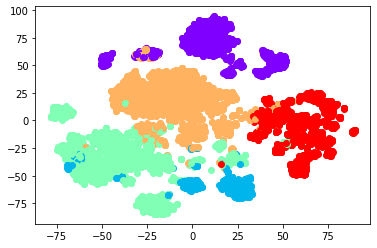
\includegraphics[width=\linewidth]{../report/image1.png}
                \caption{聚类结果}
                \label{fig:wsd}
            \end{figure}
        \end{column}
    \end{columns}
\end{frame}

\begin{frame}[allowframebreaks]{References}
    \renewcommand{\section}[2]{}
    \bibliographystyle{gbt7714-numerical}
    \bibliography{../report/references.bib}  
\end{frame}

\end{document}
